\chapter{Results}

\section{Overall MMD behaviour}

Surprisingly, we found that the behaviour of MMD was not as inconsistent for the
types of graphs extracted from proteins as was found on synthetic graphs by
\cite{o2021evaluation}. Figure \ref{fig:mmd_consistent_eps} exhibits a typical
trajectories of MMD values as different perturbation types are progressively
added to $\varepsilon$-graphs with $\varepsilon$ set to $8$\si{\angstrom}. We
can see that both the Spearman and Pearson correlation coefficients averaged
across runs are high, indicating a high correlation between the amount of
perturbation and the normalized MMD values. There is, however, an exception: the
MMD obtained from the degree histogram does not behave as expected, and is very
sensitive to the addition of edges and decreases in value as more and more edges
are added. We expect that this pathology is not very common in real models and
that this can be easily detected manually.

The overall influence of the kernel on MMD's behaviour subject to
perturbations such as Gaussian Noise, can be seen in Figure \ref{fig:mmd_effect_kernel}. We can
see that for low values of $\sigma$ (the hyperparameter of the Gaussian kernel,
see Section \ref{sec:kernels}) and for the linear kernel, MMD values behave as
desired. However, unpredictable patterns emerge when increasing $\sigma$ and the
kernel matrices can ``saturate'' quite easily. This can have quite unpredictable
behaviours: in the case of the degree histogram or the clustering histogram,
this results in an overly sensitive kernel, while the clustering histogram
remains oblivious to large amounts of perturbation.

$k$-NN graphs seem to behave similarly to $\varepsilon$-graphs, in that they are
able to detect perturbations - see Figure \ref{}. However, they are extremely
sensitive to Gaussian noise (see upper left pane of Figure \ref{}). Presumably, this is
because very small amounts of noise ($<4$\si{\angstrom}) affect the direct local
neighbourhood of each node very significantly in such a way that the resulting
$k$-NN graph is rapidly disrupted, which is not necessarily the case with other
perturbations.


\begin{figure}
  \centering
  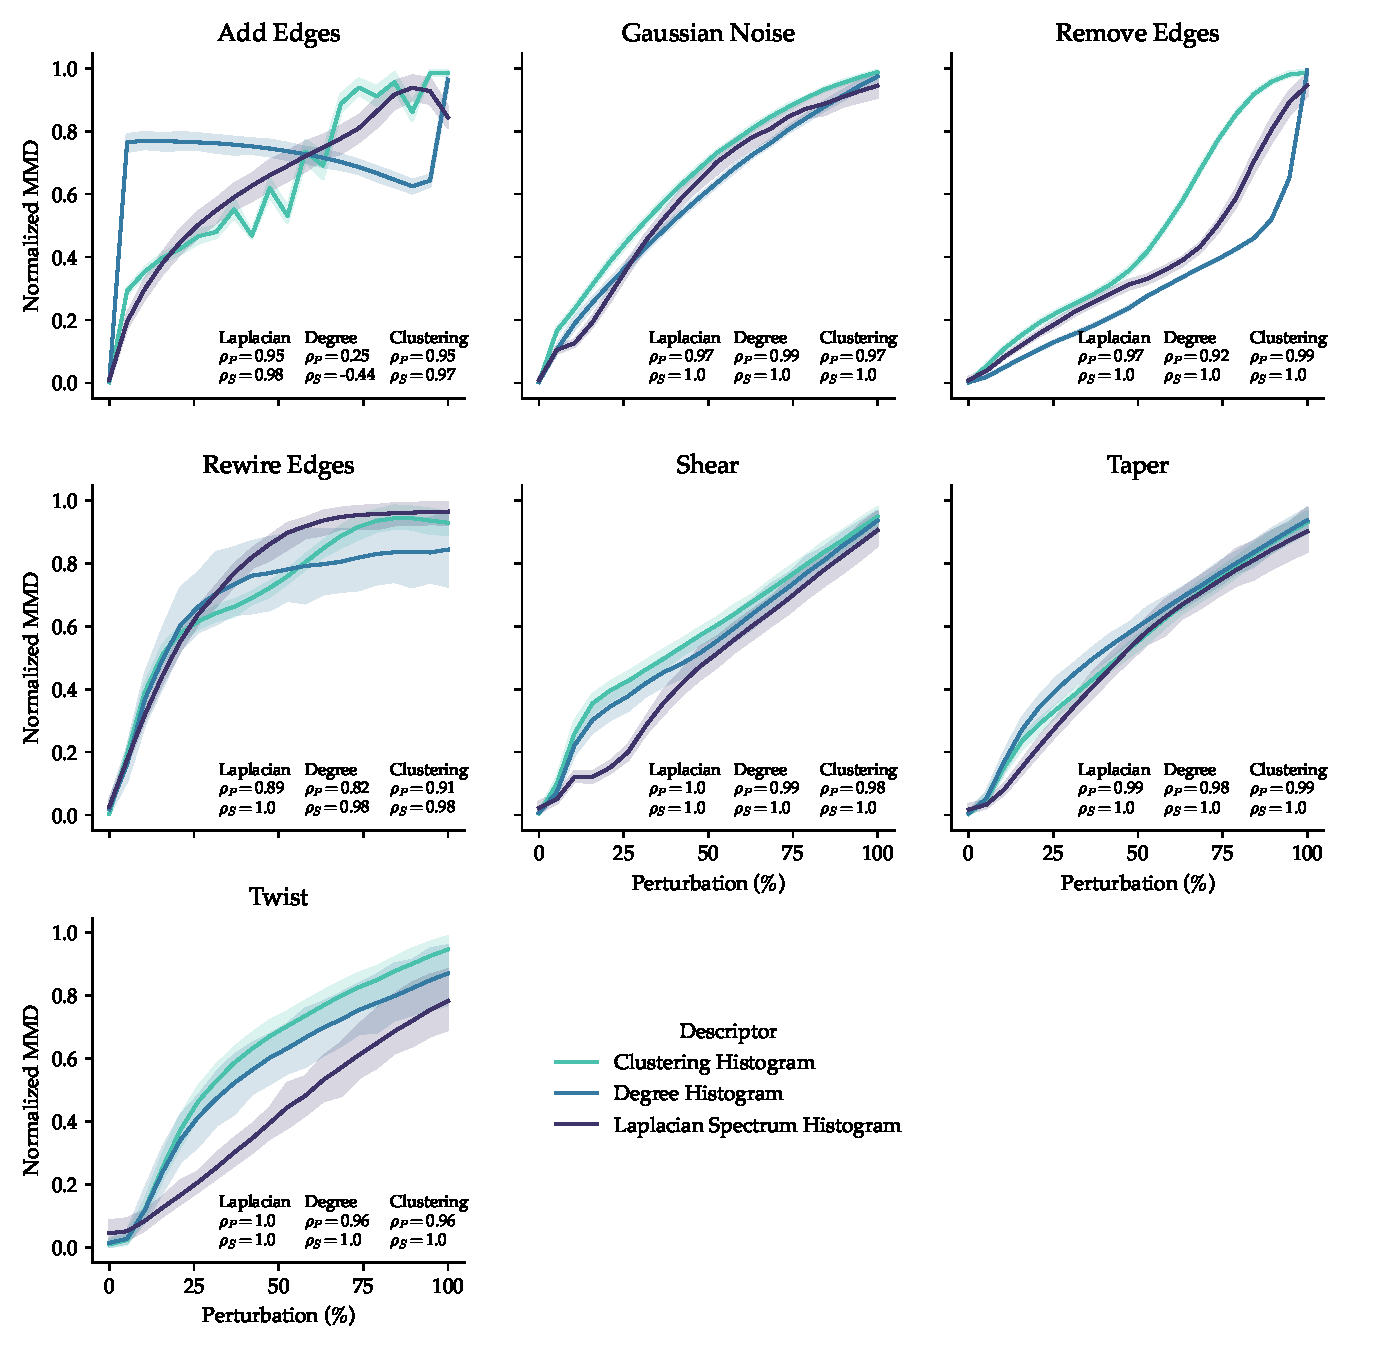
\includegraphics[width=\textwidth]{./figures/results/res_1_1.pdf}
  \caption{MMD vs. Perturbation (in \%) for various graph descriptors of the 8\si{\angstrom}-graphs under different perturbations regimes. The kernel
    used to obtain these graphs is the RBF Kernel with bandwidth 0.01.
    $\rho_{S}$: average Spearman correlation coefficient across runs.
    $\rho_{P}$: average Pearson correlation coefficient across runs.}
  \label{fig:mmd_consistent_eps}
\end{figure}


\begin{figure}
  \centering
  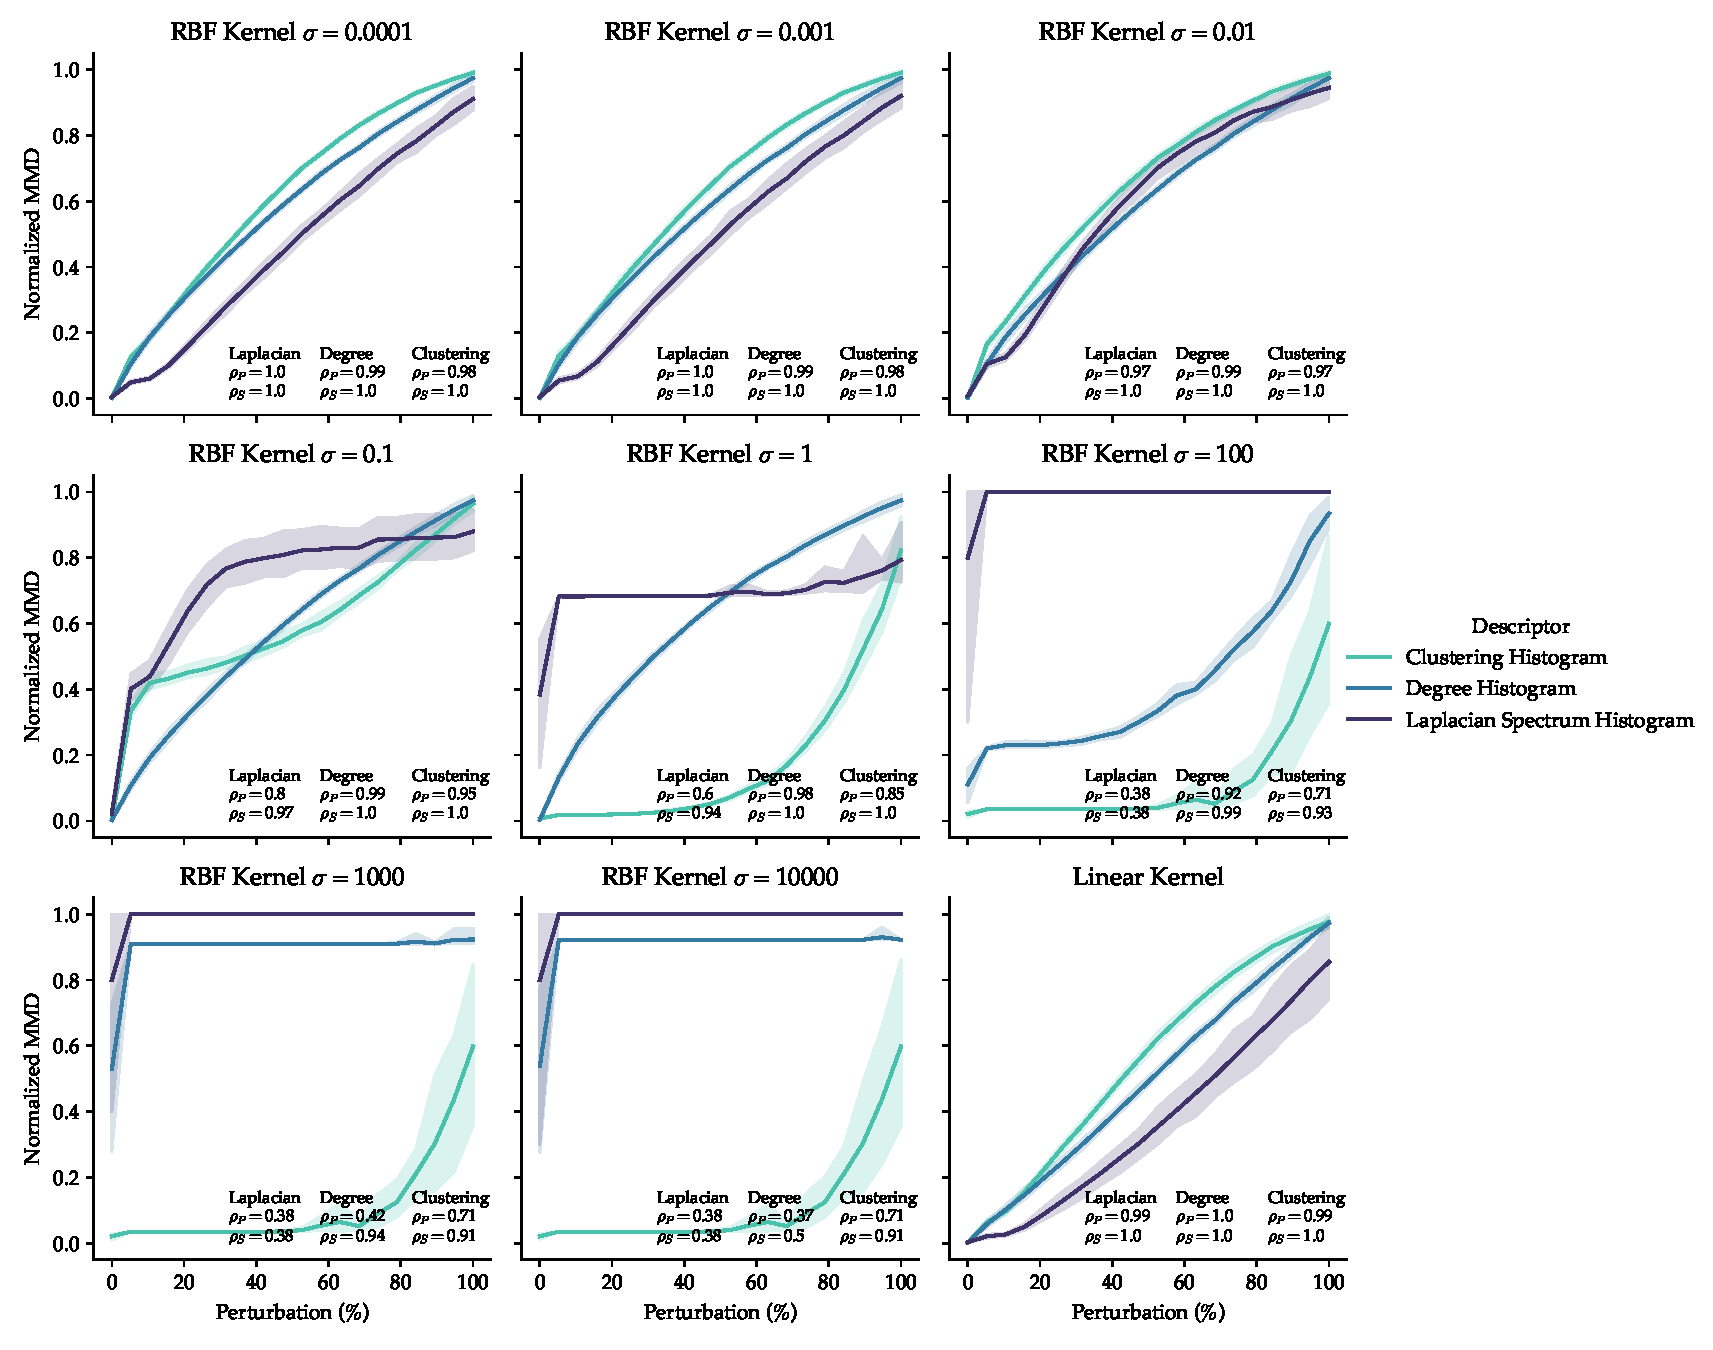
\includegraphics[width=\textwidth]{./figures/results/res_1_2.pdf}
  \caption{MMD vs. Gaussian Noise Perturbation (in \%) for various graph descriptors of the
    8\si{\angstrom}-graphs. The kernel here is shown on top of each subplots.}
  \label{fig:mmd_effect_kernel}
\end{figure}


% MMD is quite stable, somewhat contradicts what obray is saying. Maybe due to
% the different nature of the graphs.

\section{Influence of the representation on the sensitivity to perturbations}

We move on to discuss the sensitivity of the extracted graph representation to
the perturbations applied. For this analysis, we will only focus on
perturbations applied to the underlying point cloud of the graph. Specifically,
we investigate how the parameters used to extract the graph affect the
sensitivity of the resulting MMD values to the pertubation.

\begin{figure}
  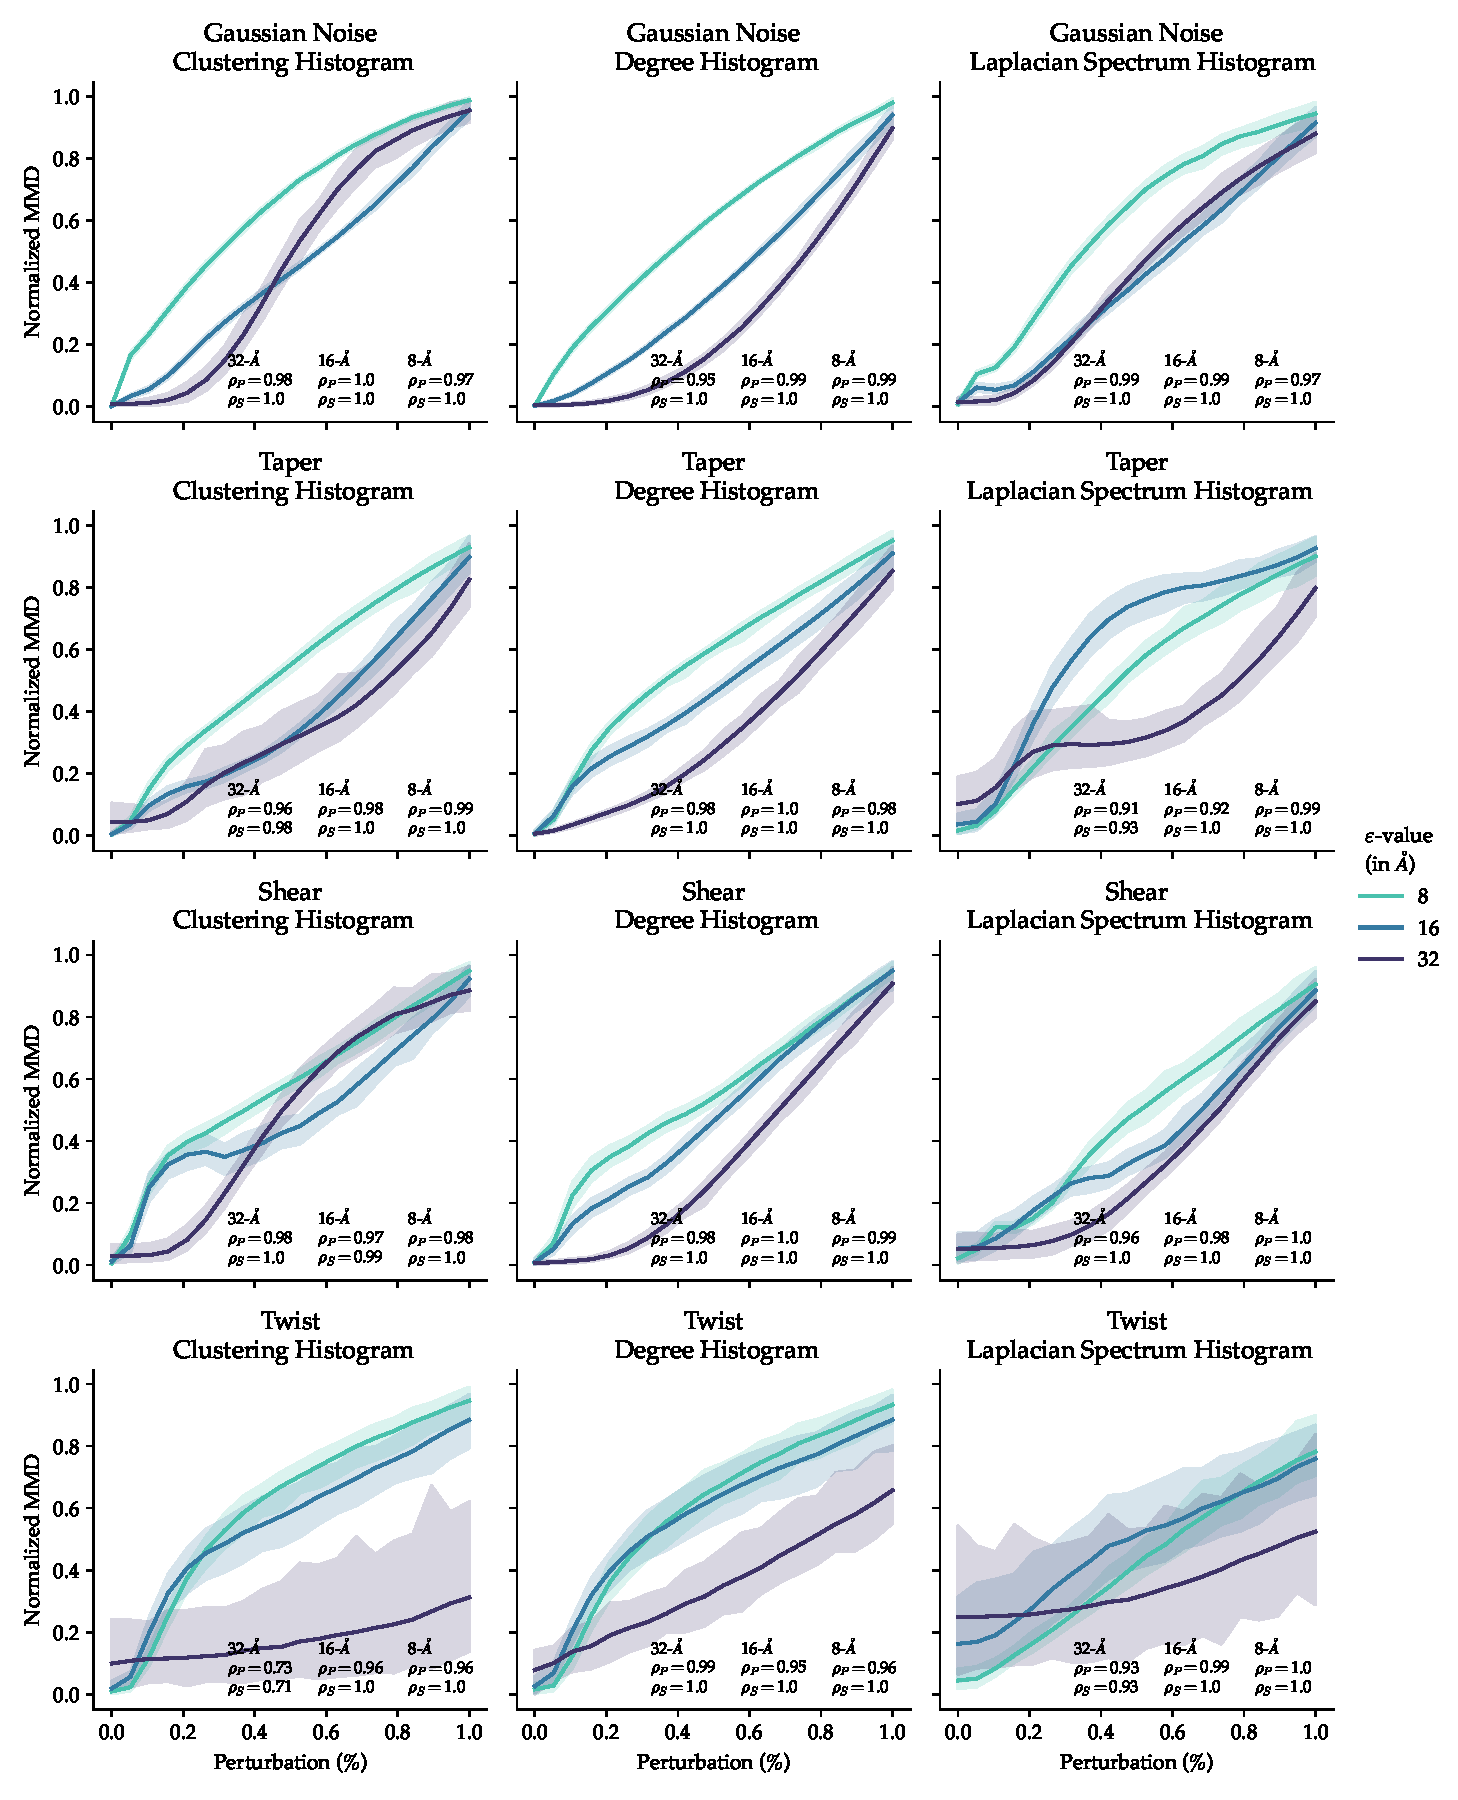
\includegraphics[width=\textwidth]{./figures/results/res_2.pdf}
\end{figure}

\section{Protein-specific descriptors}

% Scale dependent!!

\section{Topological descriptors and kernels}

\section{Runtime}

One of the desiderata of MMD is computation time (see Section \ref{sec:evalproblem}).

\begin{table}
  \centering
  \begin{tabular}{lll}
    \toprule
    \textbf{Operation} &  \textbf{Execution Time} \\
    \midrule
    Vietoris-Rips Filtration & \\
    Vietoris-Rips Filtration & \\
    \bottomrule
  \end{tabular}
  \caption{Runtime and computational complexity of the various elements of the pipeline}
  \label{tab:descriptor_function_setup}
\end{table}


% Scale FREE!!

% \section{Fixed-Length Vectors}

% \subsection{Domain agnostic descriptors}

% \subsection{Protein-specific descriptors}

% \subsection{Embeddings}

% \section{Graph Kernels}

% \subsection{Weisfeiler-Lehmann}

% \section{Topological Representations and Kernels}

% \subsection{Persistence Fisher Kernel}

\section{Summary}
